Le Morton index, également connu sous le nom de code Z, est une technique d'encodage spatiale utilisée dans le contexte de l'implicit tiling. Cette méthode permet de convertir des coordonnées multidimensionnelles en une valeur unidimensionnelle tout en préservant la proximité spatiale des points. Dans le cas de Cesium, le Morton index facilite le découpage et l'organisation hiérarchique des tuiles, rendant plus efficace la gestion et le rendu des grandes quantités de données géospatiales. En encodant les coordonnées des tuiles dans une structure arborescente, le Morton index permet une récupération rapide des tuiles nécessaires pour afficher une vue spécifique, optimisant ainsi les performances et la fluidité de la visualisation.

Il y a plusieurs opérations sur les indexes de Morton qui sont nécessaires pour la gestion des tuiles. Ces opérations sont les suivantes :

\begin{itemize}
    \item Convertir des coordonnées (X, Y, Level) en un index de Morton.
    \item Convertir un index de Morton en des coordonnées (X, Y, Level).
    \item Obtenir les 4 indexes enfants d'un index de Morton.
    \item Obtenir le nombre de bits nécessaires pour encoder un index de Morton.
\end{itemize}

\subsection*{Conversion de coordonnées en index de Morton}

Pour convertir des coordonnées (X, Y, Level) en un index de Morton, nous devons les \textit{intercaler} pour former un seul entier. L'intercalation des bits est une technique qui consiste à mélanger les bits de deux entiers pour former un index de Morton. Supposons que nous ayons deux entiers \( X \) et \( Y \), et que nous voulons les combiner en un seul entier \( Zz \) en intercalant leurs bits.

1. \textbf{Représentation binaire}

   Tout d'abord, convertissons \( X \) et \( Y \) en leurs représentations binaires :
   \[
   X = x_n x_{n-1} \ldots x_1 x_0
   \]
   \[
   Y = y_n y_{n-1} \ldots y_1 y_0
   \]

2. \textbf{Intercalage des bits}

   Ensuite, nous intercalons les bits de \( X \) et \( Y \) pour obtenir \( Z \). Le bit \( i \) de \( X \) sera placé dans la position \( 2i \) de \( Z \), et le bit \( i \) de \( y \) sera placé dans la position \( 2i + 1 \) de \( z \). De plus, l'index de Morton dépend du niveau de profondeur de la tuile. Le nombre de bits nécessaires pour encoder un index de Morton est donc égal à \(2 \times \text{level}\).

   Formulons cela mathématiquement :
   \[
   Z = \text{interleave}(x, y) = z_{2n+1} z_{2n} z_{2n-1} \ldots z_1 z_0
   \]
   où
   \[
   z_{2i} = x_i \quad \text{et} \quad z_{2i+1} = y_i \quad \text{pour} \quad i = 0, 1, \ldots, n \quad \text{avec} \quad n = 2 \times {level}
   \]

3. \textbf{Exemple}

   Prenons un exemple simple avec \( x = 5 \) et \( y = 3 \). En binaire, nous avons :
   \[
   x = 101_2 \quad \text{et} \quad y = 011_2
   \]

   Intercalons les bits :
   \[
   z = 011011_2
   \]

   En décimal, cela donne :
   \[
   z = 27_{10}
   \]

Ainsi, l'index de Morton pour \( x = 5 \) et \( y = 3 \) est \( 27 \).

\begin{figure}[H]
    \centering
    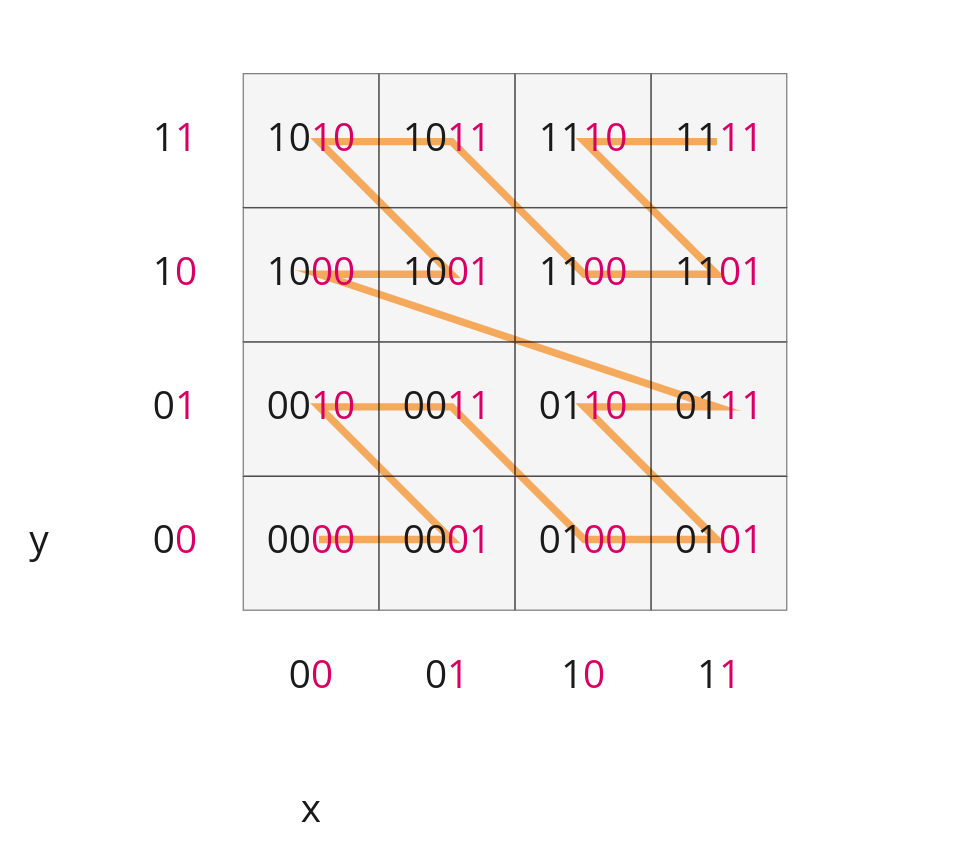
\includegraphics[width=0.6\textwidth]{assets/figures/global-to-local-xy.png}
    \caption{Indexes X Y vers index de Morton \cite{availability-gh}}
    \label{fig:xy-morton}
\end{figure}

\subsection*{Conversion d'un index de Morton en coordonnées}

Le processus inverse du \textit{interleaving bits} consiste à séparer les bits d'un index de Morton \( Z \) pour récupérer les deux entiers \( X \) et \( X \).

1. \textbf{Représentation binaire} :

   Supposons que nous avons un entier \( Z \) et que nous voulons en extraire les deux entiers \( X \) et \( Y \). Représentons \( Z \) en binaire :
   \[
   Z = z_{2n+1} z_{2n} z_{2n-1} \ldots z_1 z_0
   \]

2. \textbf{Séparation des bits} :

   Nous séparons les bits de \( Z \) pour reconstruire \( X \) et \( Y \). Les bits pairs de \( Z \) formeront \( X \), et les bits impairs de \( Z \) formeront \( Y \).

   Formulons cela mathématiquement :
   \[
   X = x_n x_{n-1} \ldots x_1 x_0
   \]
   \[
   Y = y_n y_{n-1} \ldots y_1 y_0
   \]

   où
   \[
   x_i = z_{2i} \quad \text{et} \quad y_i = z_{2i+1} \quad \text{pour} \quad i = 0, 1, \ldots, n \quad \text{avec} \quad n = 2 \times {level}
   \]

3. \textbf{Exemple} :

   Reprenons le dernier exemple avec \( Z = 27 \). En binaire, nous avons :
   \[
   Z = 011011_2
   \]

   Séparons les bits pour obtenir \( X \) et \( Y \) :
   \[
   X = z_{4}z_{2}z_{0} = 101_2 = 5_{10}
   \]
   \[
   Y = z_{5}z_{3}z_{1} = 011_2 = 3_{10}
   \]

Ainsi, les entiers \( X \) et \( Y \) extraits de l'index de Morton \( Z = 27 \) sont respectivement \( 5 \) et \( 3 \).

\subsection*{Obtention des indexes enfants}

Pour trouver les indexes enfants d'un index de Morton, nous devons simplement effectuer un décalage de 2 bits vers la gauche de l'index de Morton puis ajouter l'index de l'enfant voulu (de 0 à 3).

Par exemple, pour obtenir l'index de Morton de l'enfant 2 de l'index de Morton 27, nous effectuons les opérations suivantes :

\[
27 = 011011_2 \quad \Rightarrow \quad 01101100_2 = 108_{10}
\]

\[
108 + 2 = 110_{10} = 01101110_2
\]

Ainsi, l'index de Morton de l'enfant 2 de l'index de Morton 27 est 110.

Une distinction qui se trouve parfois pratique est la distinction d'un index local versus un index global. Un index global est un index de Morton qui représente une tuile sur l'entièreté du Tileset, en comptant donc depuis l'index 0 du level 0. Tandis qu'un index local est un index de Morton qui représente une tuile avec pour référence l'index 0 du subtree.

\begin{figure}[H]
    \centering
    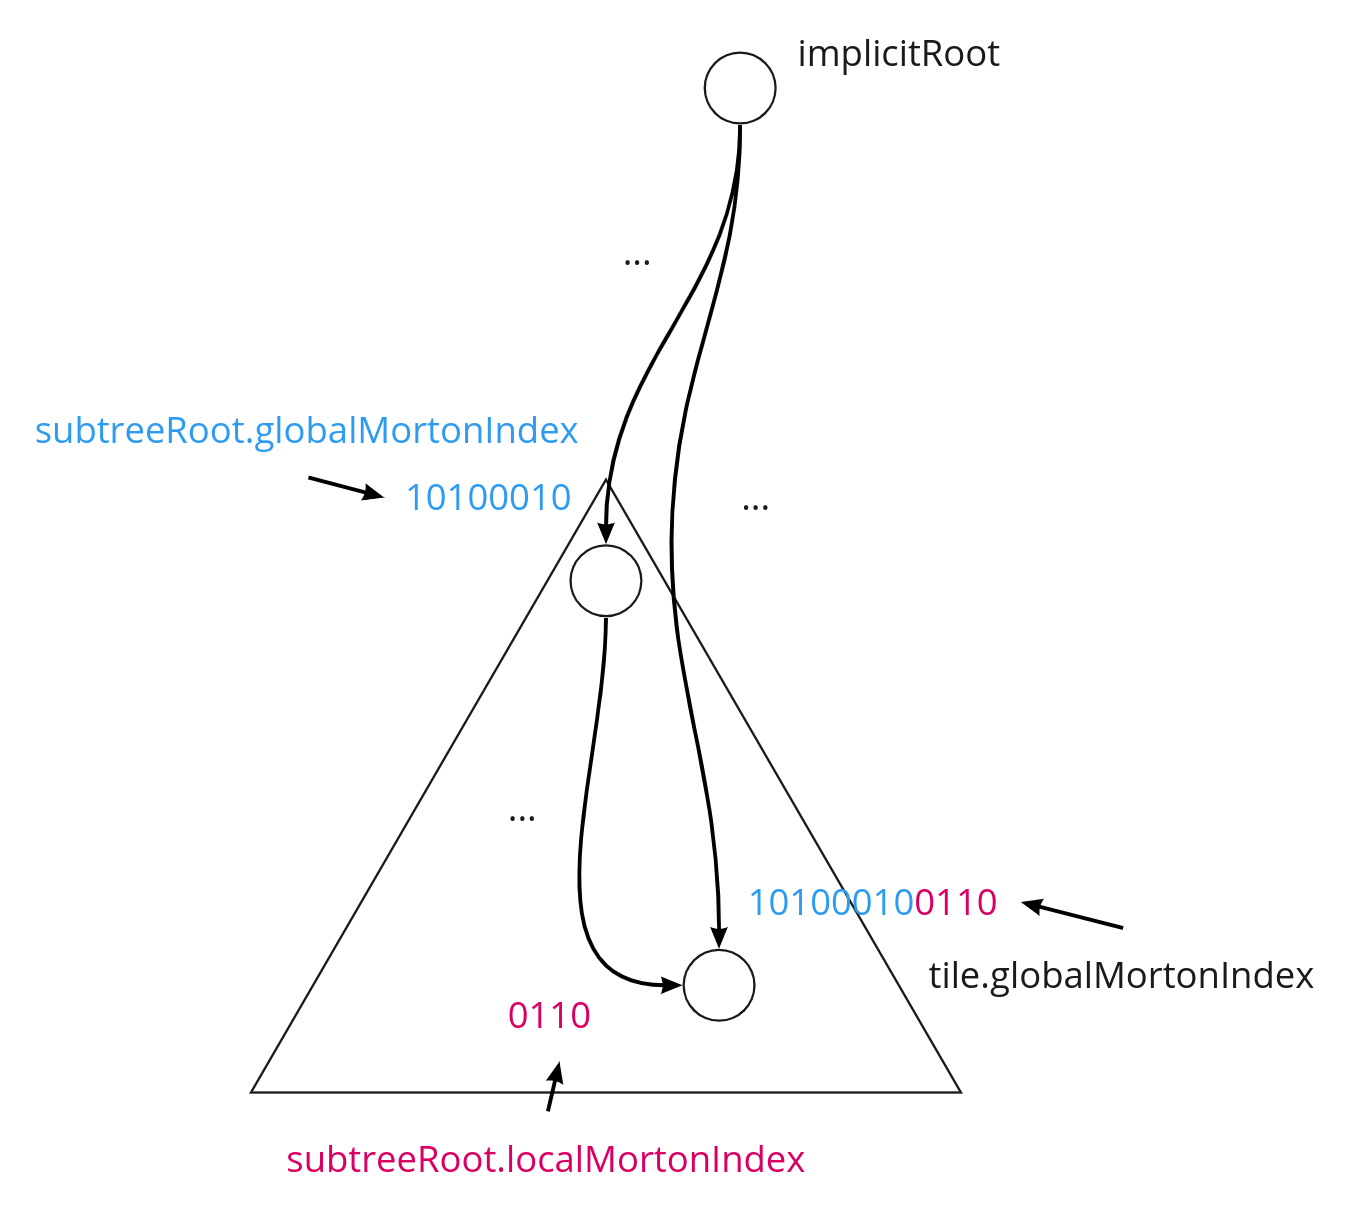
\includegraphics[width=0.8\textwidth]{assets/figures/global-to-local-morton.png}
    \caption{Index local et index global \cite{availability-gh}}
    \label{fig:xy-morton}
\end{figure}